\documentclass[9pt]{beamer}
\usepackage[utf8]{inputenc}
\usefonttheme{serif} 
\usefonttheme{structuresmallcapsserif} 
\usepackage{hyperref}
\hypersetup{
    colorlinks=true,
    linkcolor=blue,
    filecolor=magenta,
    urlcolor=cyan,
}

\usetheme{Luebeck}
%\usepackage{media9}
%\usepackage{animate}
\usepackage{multimedia}
\usepackage{textpos} 

\addtobeamertemplate{frametitle}{}{%
    \begin{textblock*}{100mm}(11.75cm,-0.86cm)
        
\includegraphics[height=0.86cm,width=0.86cm]{HIPlogo.png}
    \end{textblock*}
    }
\addtobeamertemplate{frametitle}{}{%
    \begin{textblock*}{100mm}(10.89cm,-0.86cm)
        
\includegraphics[height=0.86cm,width=0.86cm]{HYlogo.jpg}
    \end{textblock*}}
\addtobeamertemplate{frametitle}{}{%
    \begin{textblock*}{100mm}(10.03cm,-0.86cm)
        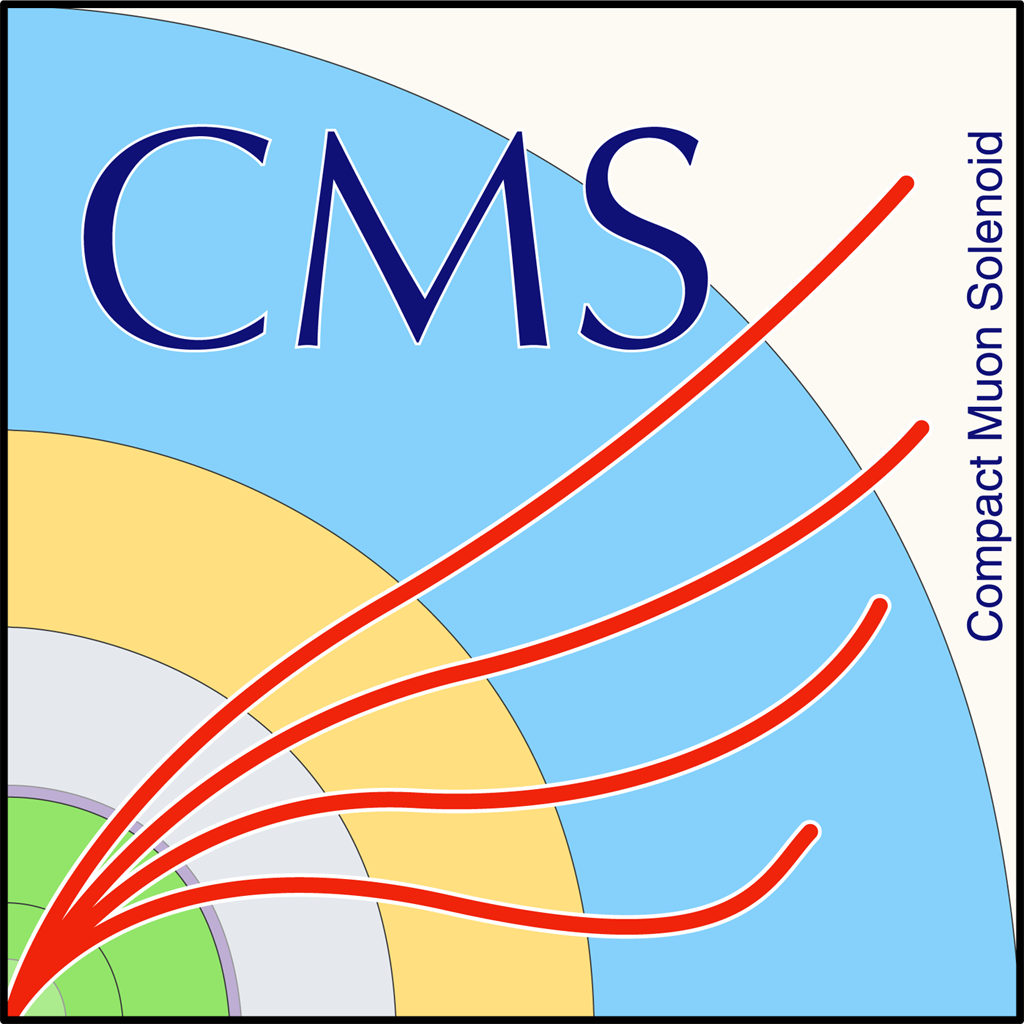
\includegraphics[height=0.86cm,width=0.86cm]{CMSlogo.png}
    \end{textblock*}}

\definecolor{ao}{rgb}{0.0, 0.5, 0.0}
\definecolor{darkgreen}{rgb}{0.0, 0.2, 0.13}
\definecolor{ferngreen}{rgb}{0.31, 0.47, 0.26}
    
\usecolortheme[named=ferngreen]{structure}
\beamertemplatenavigationsymbolsempty
\setbeamertemplate{bibliography item}[text]
\title[C17 (UL ReReco) hot zones]{C17 (UL ReReco) hot zones}
%\subtitle{JERC meeting 26th Feb 2018}
\author{Hannu Siikonen}
\institute{Helsinki Institute of Physics \\ \vspace{0.25cm} Instructor Adj.~Prof.~Mikko~Voutilainen}

\date{\today}

\setbeamersize{text margin left=5pt,text margin right=5pt}
\setlength{\labelsep}{12pt}

\begin{document}

\begin{frame}[t]
\titlepage
\end{frame}

\begin{frame}[t]{Motivation and Practicalities}
\begin{columns}[T]
\begin{column}{\textwidth}
\begin{itemize}
 \item Some parts of the detector might not function optimally
 \item This is seen as an excess (hot zone) or lack (cold zone) of jets
 \item Typically, cold zones are modeled well in MC, but hot zones are not
 \item In precision studies, it makes sense to exclude detector patches that are displayed as such hot zones
 \item The patches for the hot zones are found in the hotjets-*.root file, in the histogram h2hotfilter (also the raw histogram is provided)
 \item In h2hotfilter, a value above zero indicates a hot zone
 \item For simplicity, it can be advisable to use the full-year filter map (which is a sum over all the era filters)
 \item ZeroBias and JetHT samples are used for Data
 \item Standard (flat) QCD + SingleNeutrino samples are used for MC
\end{itemize}
\end{column}
\end{columns}
\end{frame}

\begin{frame}[t]{Methodology and Formulas}
\begin{columns}[T]
\begin{column}{\textwidth}
\begin{itemize}
 \item Fluctuations are studied within bins corresponding to HCAL towers\footnote{Binning picked from L2Relative JEC file}
 \item In one $\eta$ strip of bins, we compute the binwise mean ($\mu$) and sample variance ($s$) of jets passing the jet ID:
 \begin{eqnarray}
     \mu_{\eta}^{trg} &=& \frac{\sum_{i=1}^{N_\phi} N_{jet,\eta}^{i,trg}}{N_\phi} \\
     s_{\eta}^{trg} &=& \sqrt{\frac{\sum_{i=1}^{^{N_\phi}}\left(N_{jet,\eta}^{i,trg}-\mu\right)^2}{N_\phi-1}}
 \end{eqnarray}
 \item The binwise fluctuations are plotted w.r.t. $\sigma$ in the $\eta$ strips with more than 14 of the 72 $\phi$ bins are activated (not empty)
 \item The binwise fluctuations are plotted w.r.t. $\mu$ in the $\eta$ strips where $\mu > \sigma$
 \item We define the following function to help on the next slide
     \begin{equation}
     f(x) =
  \begin{cases}
    0, &\quad\text{if } x < 3\\
    x, &\quad\text{else}
  \end{cases}
 \end{equation}
\end{itemize}
\end{column}
\end{columns}
\end{frame}

\begin{frame}[t]{Calculating the Filter by Trigger Combination}
\begin{columns}[T]
\begin{column}{\textwidth}
\begin{itemize}
 \item Within a single $\eta-\phi$ bin, the $3\sigma+$ fluctuations are summed up from the different triggers (that are usable for the given $|\eta|$ value):
 \begin{equation}
     var_{tot}= \frac{1}{N_{Trg}^{Avail}}\sum_{trg=1}^{N_{Trg}^{Avail}} f\left(\frac{\left(N_{jet,\eta}^{i_\phi,trg} - \mu_\eta^{trg}\right)}{s_\eta^{trg}}\right)
 \end{equation}
    \item The value of $N_{Trg}^{Avail}$ must be determined by looking which triggers provide enough jet statistics up to the current $\eta$ value
    \item Threshold values for $var_{tot}$ to become filter patches are determined as a function of $N_{Trg}^{Avail}$:
        \begin{equation}
            var_{tot}^{thresh} =
     \begin{cases}
       4, &\quad\text{if } N_{Trg}^{Avail} = 1\\
       3, &\quad\text{if } N_{Trg}^{Avail} = 2,3\\
       2, &\quad\text{if } N_{Trg}^{Avail} = 4,5,6\\
       1.5, &\quad\text{if } N_{Trg}^{Avail} = 7,8\\
       1, &\quad\text{else}
     \end{cases}
        \end{equation}
    \item In practice, this means that for a single trigger we require $4\sigma$, for 2 or 3 triggers in average $3\sigma$ per trigger, etc. $\rightarrow$ sensible trigger combination
\end{itemize}
\end{column}
\end{columns}
\end{frame}

\begin{frame}[t]{HLT\_ZeroBias Data}
\begin{columns}[T]
  \begin{column}{.5\textwidth}
  \includegraphics[width=\linewidth]{../pdf/data_DiffPerMean_jt0.pdf}
  \end{column}
  \begin{column}{.5\textwidth}
  \includegraphics[width=\linewidth]{../pdf/data_DiffPerVar_jt0.pdf}
  \end{column}
\end{columns}
\end{frame}

\begin{frame}[t]{HLT\_PFJet40 Data}
\begin{columns}[T]
  \begin{column}{.5\textwidth}
  \includegraphics[width=\linewidth]{../pdf/data_DiffPerMean_jt40.pdf}
  \end{column}
  \begin{column}{.5\textwidth}
  \includegraphics[width=\linewidth]{../pdf/data_DiffPerVar_jt40.pdf}
  \end{column}
\end{columns}
\end{frame}

\begin{frame}[t]{HLT\_PFJet60 Data}
\begin{columns}[T]
  \begin{column}{.5\textwidth}
  \includegraphics[width=\linewidth]{../pdf/data_DiffPerMean_jt60.pdf}
  \end{column}
  \begin{column}{.5\textwidth}
  \includegraphics[width=\linewidth]{../pdf/data_DiffPerVar_jt60.pdf}
  \end{column}
\end{columns}
\end{frame}

\begin{frame}[t]{HLT\_PFJet80 Data}
\begin{columns}[T]
  \begin{column}{.5\textwidth}
  \includegraphics[width=\linewidth]{../pdf/data_DiffPerMean_jt80.pdf}
  \end{column}
  \begin{column}{.5\textwidth}
  \includegraphics[width=\linewidth]{../pdf/data_DiffPerVar_jt80.pdf}
  \end{column}
\end{columns}
\end{frame}

\begin{frame}[t]{HLT\_PFJet140 Data}
\begin{columns}[T]
  \begin{column}{.5\textwidth}
  \includegraphics[width=\linewidth]{../pdf/data_DiffPerMean_jt140.pdf}
  \end{column}
  \begin{column}{.5\textwidth}
  \includegraphics[width=\linewidth]{../pdf/data_DiffPerVar_jt140.pdf}
  \end{column}
\end{columns}
\end{frame}

\begin{frame}[t]{HLT\_PFJet200 Data}
\begin{columns}[T]
  \begin{column}{.5\textwidth}
  \includegraphics[width=\linewidth]{../pdf/data_DiffPerMean_jt200.pdf}
  \end{column}
  \begin{column}{.5\textwidth}
  \includegraphics[width=\linewidth]{../pdf/data_DiffPerVar_jt200.pdf}
  \end{column}
\end{columns}
\end{frame}

\begin{frame}[t]{HLT\_PFJet260 Data}
\begin{columns}[T]
  \begin{column}{.5\textwidth}
  \includegraphics[width=\linewidth]{../pdf/data_DiffPerMean_jt260.pdf}
  \end{column}
  \begin{column}{.5\textwidth}
  \includegraphics[width=\linewidth]{../pdf/data_DiffPerVar_jt260.pdf}
  \end{column}
\end{columns}
\end{frame}

\begin{frame}[t]{HLT\_PFJet320 Data}
\begin{columns}[T]
  \begin{column}{.5\textwidth}
  \includegraphics[width=\linewidth]{../pdf/data_DiffPerMean_jt320.pdf}
  \end{column}
  \begin{column}{.5\textwidth}
  \includegraphics[width=\linewidth]{../pdf/data_DiffPerVar_jt320.pdf}
  \end{column}
\end{columns}
\end{frame}

\begin{frame}[t]{HLT\_PFJet400 Data}
\begin{columns}[T]
  \begin{column}{.5\textwidth}
  \includegraphics[width=\linewidth]{../pdf/data_DiffPerMean_jt400.pdf}
  \end{column}
  \begin{column}{.5\textwidth}
  \includegraphics[width=\linewidth]{../pdf/data_DiffPerVar_jt400.pdf}
  \end{column}
\end{columns}
\end{frame}

\begin{frame}[t]{HLT\_PFJet450 Data}
\begin{columns}[T]
  \begin{column}{.5\textwidth}
  \includegraphics[width=\linewidth]{../pdf/data_DiffPerMean_jt450.pdf}
  \end{column}
  \begin{column}{.5\textwidth}
  \includegraphics[width=\linewidth]{../pdf/data_DiffPerVar_jt450.pdf}
  \end{column}
\end{columns}
\end{frame}

\begin{frame}[t]{HLT\_PFJet500 Data}
\begin{columns}[T]
  \begin{column}{.5\textwidth}
  \includegraphics[width=\linewidth]{../pdf/data_DiffPerMean_jt500.pdf}
  \end{column}
  \begin{column}{.5\textwidth}
  \includegraphics[width=\linewidth]{../pdf/data_DiffPerVar_jt500.pdf}
  \end{column}
\end{columns}
\end{frame}

\begin{frame}[t]{Cumulative summary (P8,DATA)}
\begin{columns}[T]
  \begin{column}{.5\textwidth}
  \includegraphics[width=\linewidth]{../pdf/mc_cumulation.pdf}
  \end{column}
  \begin{column}{.5\textwidth}
  \includegraphics[width=\linewidth]{../pdf/data_cumulation.pdf}
  \end{column}
\end{columns}
\begin{itemize}
 \item Cumulative summary plots over all triggers - attempt to present the excess/deficit plots cumulated over all triggers
 \item In the $\eta$ border zones only the triggers with a sufficient amount of data is used
\end{itemize}
\end{frame}

\begin{frame}[t]{Filtered cumulative summary Data (cold, hot)}
\begin{columns}[T]
  \begin{column}{.5\textwidth}
  \includegraphics[width=\linewidth]{../pdf/data_colds.pdf}
  \end{column}
  \begin{column}{.5\textwidth}
  \includegraphics[width=\linewidth]{../pdf/data_hots.pdf}
  \end{column}
\end{columns}
\begin{itemize}
 \item The same procedure as on the previous slide, but now we emphasize noise that is significant in more than only one trigger
 \item Hot and cold zones separated
\end{itemize}
\end{frame}

\begin{frame}[t]{Filtered cumulative summary P8 (cold, hot)}
\begin{columns}[T]
  \begin{column}{.5\textwidth}
  \includegraphics[width=\linewidth]{../pdf/mc_colds.pdf}
  \end{column}
  \begin{column}{.5\textwidth}
  \includegraphics[width=\linewidth]{../pdf/mc_hots.pdf}
  \end{column}
\end{columns}
\begin{itemize}
 \item The same procedure as on the previous slide, but now we emphasize noise that is significant in more than only one trigger
 \item Hot and cold zones separated
\end{itemize}
\end{frame}

\begin{frame}[t]{Jet counts ZeroBias (P8,DATA)}
\begin{columns}[T]
  \begin{column}{.5\textwidth}
  \includegraphics[width=\linewidth]{../pdf/mc_njet_jt0.pdf}
  \end{column}
  \begin{column}{.5\textwidth}
  \includegraphics[width=\linewidth]{../pdf/data_njet_jt0.pdf}
  \end{column}
\end{columns}
\begin{itemize}
 \item Left: Pythia~8; Right: Data
 \item White patches: $3\sigma+$ downwards fluctuations for this trigger
 \item Black patches: $3\sigma+$ upwards fluctuations for this trigger
\end{itemize}
\end{frame}

\begin{frame}[t]{Jet counts JetHT40 (P8,DATA)}
\begin{columns}[T]
  \begin{column}{.5\textwidth}
  \includegraphics[width=\linewidth]{../pdf/mc_njet_jt40.pdf}
  \end{column}
  \begin{column}{.5\textwidth}
  \includegraphics[width=\linewidth]{../pdf/data_njet_jt40.pdf}
  \end{column}
\end{columns}
\begin{itemize}
 \item Left: Pythia~8; Right: Data
 \item White patches: $3\sigma+$ downwards fluctuations for this trigger
 \item Black patches: $3\sigma+$ upwards fluctuations for this trigger
\end{itemize}
\end{frame}

\begin{frame}[t]{Jet counts JetHT60 (P8,DATA)}
\begin{columns}[T]
  \begin{column}{.5\textwidth}
  \includegraphics[width=\linewidth]{../pdf/mc_njet_jt60.pdf}
  \end{column}
  \begin{column}{.5\textwidth}
  \includegraphics[width=\linewidth]{../pdf/data_njet_jt60.pdf}
  \end{column}
\end{columns}
\begin{itemize}
 \item Left: Pythia~8; Right: Data
 \item White patches: $3\sigma+$ downwards fluctuations for this trigger
 \item Black patches: $3\sigma+$ upwards fluctuations for this trigger
\end{itemize}
\end{frame}

\begin{frame}[t]{Jet counts JetHT80 (P8,DATA)}
\begin{columns}[T]
  \begin{column}{.5\textwidth}
  \includegraphics[width=\linewidth]{../pdf/mc_njet_jt80.pdf}
  \end{column}
  \begin{column}{.5\textwidth}
  \includegraphics[width=\linewidth]{../pdf/data_njet_jt80.pdf}
  \end{column}
\end{columns}
\begin{itemize}
 \item Left: Pythia~8; Right: Data
 \item White patches: $3\sigma+$ downwards fluctuations for this trigger
 \item Black patches: $3\sigma+$ upwards fluctuations for this trigger
\end{itemize}
\end{frame}

\begin{frame}[t]{Jet counts JetHT140 (P8,DATA)}
\begin{columns}[T]
  \begin{column}{.5\textwidth}
  \includegraphics[width=\linewidth]{../pdf/mc_njet_jt140.pdf}
  \end{column}
  \begin{column}{.5\textwidth}
  \includegraphics[width=\linewidth]{../pdf/data_njet_jt140.pdf}
  \end{column}
\end{columns}
\begin{itemize}
 \item Left: Pythia~8; Right: Data
 \item White patches: $3\sigma+$ downwards fluctuations for this trigger
 \item Black patches: $3\sigma+$ upwards fluctuations for this trigger
\end{itemize}
\end{frame}

\begin{frame}[t]{Jet counts JetHT200 (P8,DATA)}
\begin{columns}[T]
  \begin{column}{.5\textwidth}
  \includegraphics[width=\linewidth]{../pdf/mc_njet_jt200.pdf}
  \end{column}
  \begin{column}{.5\textwidth}
  \includegraphics[width=\linewidth]{../pdf/data_njet_jt200.pdf}
  \end{column}
\end{columns}
\begin{itemize}
 \item Left: Pythia~8; Right: Data
 \item White patches: $3\sigma+$ downwards fluctuations for this trigger
 \item Black patches: $3\sigma+$ upwards fluctuations for this trigger
\end{itemize}
\end{frame}

\begin{frame}[t]{Jet counts JetHT260 (P8,DATA)}
\begin{columns}[T]
  \begin{column}{.5\textwidth}
  \includegraphics[width=\linewidth]{../pdf/mc_njet_jt260.pdf}
  \end{column}
  \begin{column}{.5\textwidth}
  \includegraphics[width=\linewidth]{../pdf/data_njet_jt260.pdf}
  \end{column}
\end{columns}
\begin{itemize}
 \item Left: Pythia~8; Right: Data
 \item White patches: $3\sigma+$ downwards fluctuations for this trigger
 \item Black patches: $3\sigma+$ upwards fluctuations for this trigger
\end{itemize}
\end{frame}

\begin{frame}[t]{Jet counts JetHT320 (P8,DATA)}
\begin{columns}[T]
  \begin{column}{.5\textwidth}
  \includegraphics[width=\linewidth]{../pdf/mc_njet_jt320.pdf}
  \end{column}
  \begin{column}{.5\textwidth}
  \includegraphics[width=\linewidth]{../pdf/data_njet_jt320.pdf}
  \end{column}
\end{columns}
\begin{itemize}
 \item Left: Pythia~8; Right: Data
 \item White patches: $3\sigma+$ downwards fluctuations for this trigger
 \item Black patches: $3\sigma+$ upwards fluctuations for this trigger
\end{itemize}
\end{frame}

\begin{frame}[t]{Jet counts JetHT400 (P8,DATA)}
\begin{columns}[T]
  \begin{column}{.5\textwidth}
  \includegraphics[width=\linewidth]{../pdf/mc_njet_jt400.pdf}
  \end{column}
  \begin{column}{.5\textwidth}
  \includegraphics[width=\linewidth]{../pdf/data_njet_jt400.pdf}
  \end{column}
\end{columns}
\begin{itemize}
 \item Left: Pythia~8; Right: Data
 \item White patches: $3\sigma+$ downwards fluctuations for this trigger
 \item Black patches: $3\sigma+$ upwards fluctuations for this trigger
\end{itemize}
\end{frame}

\begin{frame}[t]{Jet counts JetHT450 (P8,DATA)}
\begin{columns}[T]
  \begin{column}{.5\textwidth}
  \includegraphics[width=\linewidth]{../pdf/mc_njet_jt450.pdf}
  \end{column}
  \begin{column}{.5\textwidth}
  \includegraphics[width=\linewidth]{../pdf/data_njet_jt450.pdf}
  \end{column}
\end{columns}
\begin{itemize}
 \item Left: Pythia~8; Right: Data
 \item White patches: $3\sigma+$ downwards fluctuations for this trigger
 \item Black patches: $3\sigma+$ upwards fluctuations for this trigger
\end{itemize}
\end{frame}

\begin{frame}[t]{Jet counts JetHT500 (P8,DATA)}
\begin{columns}[T]
  \begin{column}{.5\textwidth}
  \includegraphics[width=\linewidth]{../pdf/mc_njet_jt500.pdf}
  \end{column}
  \begin{column}{.5\textwidth}
  \includegraphics[width=\linewidth]{../pdf/data_njet_jt500.pdf}
  \end{column}
\end{columns}
\begin{itemize}
 \item Left: Pythia~8; Right: Data
 \item White patches: $3\sigma+$ downwards fluctuations for this trigger
 \item Black patches: $3\sigma+$ upwards fluctuations for this trigger
\end{itemize}
\end{frame}

\end{document}
